\documentclass[12pt,a4paper]{article}

%% ── Encoding & Language ─────────────────────────────────────────────────────
\usepackage[utf8]{inputenc}
\usepackage[T1]{fontenc}
\usepackage[brazil]{babel}
\usepackage{lmodern}

%% ── Layout ──────────────────────────────────────────────────────────────────
\usepackage[top=2.5cm, bottom=2.5cm, left=2.8cm, right=2.8cm]{geometry}
\usepackage{setspace}
\setstretch{1.15}

%% ── Graphics & Color ────────────────────────────────────────────────────────
\usepackage{graphicx}
\usepackage[table,dvipsnames]{xcolor}
\definecolor{azulescuro}{RGB}{30,60,100}
\definecolor{azulmedio}{RGB}{52,100,160}
\definecolor{azulclaro}{RGB}{220,235,250}
\definecolor{verdeclaro}{RGB}{220,245,220}
\definecolor{vermelho}{RGB}{180,30,30}
\definecolor{laranja}{RGB}{200,100,20}
\definecolor{amareloclaro}{RGB}{255,252,220}
\definecolor{cinzabg}{RGB}{248,248,250}

%% ── Tables ──────────────────────────────────────────────────────────────────
\usepackage{booktabs}
\usepackage{tabularx}
\usepackage{colortbl}
\usepackage{multirow}
\usepackage{array}

%% ── Code listings ───────────────────────────────────────────────────────────
\usepackage{listings}
\lstset{
  basicstyle=\ttfamily\small,
  backgroundcolor=\color{cinzabg},
  frame=single, framerule=0.5pt, rulecolor=\color{azulmedio},
  breaklines=true, breakatwhitespace=true,
  numbers=left, numberstyle=\tiny\color{gray},
  keywordstyle=\color{azulmedio}\bfseries,
  commentstyle=\color{gray}\itshape,
  stringstyle=\color{OliveGreen!80!black},
  tabsize=4,
  captionpos=b
}

%% ── Boxes ───────────────────────────────────────────────────────────────────
\usepackage[most]{tcolorbox}
\tcbuselibrary{skins,breakable}

\newtcolorbox{notabox}[1][]{
  enhanced, breakable,
  colback=azulclaro!40, colframe=azulmedio,
  fonttitle=\bfseries\small, title=Nota,
  top=4pt, bottom=4pt, left=8pt, right=8pt,
  #1
}

\newtcolorbox{codigobox}[1][]{
  enhanced, breakable,
  colback=cinzabg, colframe=azulescuro,
  fonttitle=\bfseries\small,
  top=4pt, bottom=4pt, left=8pt, right=8pt,
  #1
}

\newtcolorbox{equacaobox}[1][]{
  enhanced, breakable,
  colback=amareloclaro, colframe=laranja,
  top=6pt, bottom=6pt, left=12pt, right=12pt,
  #1
}

\newtcolorbox{atencaobox}[1][]{
  enhanced,
  colback=red!8, colframe=vermelho,
  fonttitle=\bfseries\small, title=Aten\c{c}\~ao,
  top=4pt, bottom=4pt, left=8pt, right=8pt,
  #1
}

%% ── Section styling ─────────────────────────────────────────────────────────
\usepackage{titlesec}
\titleformat{\section}
  {\Large\bfseries\color{azulescuro}}{\thesection.}{0.6em}{}
  [{\color{azulmedio}\titlerule[1.2pt]}]
\titleformat{\subsection}
  {\large\bfseries\color{azulmedio}}{\thesubsection.}{0.5em}{}
\titleformat{\subsubsection}
  {\normalsize\bfseries\color{azulescuro}}{\thesubsubsection.}{0.4em}{}

%% ── Header / footer ─────────────────────────────────────────────────────────
\usepackage{fancyhdr}
\pagestyle{fancy}
\fancyhf{}
\fancyhead[L]{\small\color{azulmedio} AEB -- Camada de Percep\c{c}\~ao}
\fancyhead[R]{\small\color{azulmedio} Modelagem Simulink}
\fancyfoot[C]{\small\thepage}
\renewcommand{\headrulewidth}{0.5pt}

%% ── Math ────────────────────────────────────────────────────────────────────
\usepackage{amsmath}
\usepackage{amssymb}

%% ── Hyperlinks ──────────────────────────────────────────────────────────────
\usepackage[colorlinks=true, linkcolor=azulmedio, urlcolor=azulmedio,
            citecolor=azulmedio, pdftitle={AEB Percepcao Simulink},
            pdfauthor={AEB Team}]{hyperref}

%% ── Misc ────────────────────────────────────────────────────────────────────
\usepackage{float}
\usepackage{caption}
\captionsetup{font=small, labelfont={bf,color=azulescuro}, labelsep=period}
\usepackage{enumitem}
\setlist[itemize]{itemsep=2pt, topsep=4pt}

%% ════════════════════════════════════════════════════════════════════════════
\begin{document}

%% ── Title page ──────────────────────────────────────────────────────────────
\begin{titlepage}
  \begin{center}
    \vspace*{1.5cm}
    {\color{azulescuro}\rule{\linewidth}{2pt}}\\[0.4cm]
    {\Huge\bfseries\color{azulescuro} Sistema AEB}\\[0.3cm]
    {\LARGE\bfseries\color{azulmedio} Modelagem da Camada de Percep\c{c}\~ao}\\[0.2cm]
    {\large\color{azulmedio} Modelo Simulink Independente --- AEB\_Perception.slx}\\[0.2cm]
    {\color{azulescuro}\rule{\linewidth}{2pt}}

    \vspace{1.8cm}
    \begin{tcolorbox}[enhanced,
      colback=azulclaro!30, colframe=azulmedio,
      width=0.85\linewidth, halign=center,
      top=10pt, bottom=10pt]
      \large\bfseries\color{azulescuro}
      Documento T\'ecnico de Modelagem\\[0.3cm]
      \normalsize\normalfont\color{black}
      Especifica\c{c}\~ao dos subsistemas Radar, LiDAR,\\
      Fus\~ao Sensorial e Detec\c{c}\~ao de Falha\\
      conforme implementado em \texttt{aeb\_perception.c}
    \end{tcolorbox}

    \vspace{1.5cm}
    \begin{tabular}{ll}
      \textbf{Vers\~ao:}    & 1.0 \\[4pt]
      \textbf{Data:}        & Mar\c{c}o de 2026 \\[4pt]
      \textbf{Ferramenta:}  & MATLAB/Simulink R2025b \\[4pt]
      \textbf{Refer\^encia:} & \texttt{modeling/c\_embedded/src/aeb\_perception.c} \\[4pt]
      \textbf{Protocolo:}   & Euro NCAP AEB C2C v4.3 \\
    \end{tabular}

    \vfill
    {\color{azulescuro}\rule{\linewidth}{1pt}}\\[0.3cm]
    {\small\color{gray}
      Frenagem Aut\^onoma de Emerg\^encia (AEB) --- Projeto de P\'os-Gradua\c{c}\~ao\\
      Modelagem, Simula\c{c}\~ao e Valida\c{c}\~ao SIL
    }
  \end{center}
\end{titlepage}

%% ── TOC ─────────────────────────────────────────────────────────────────────
\tableofcontents
\newpage

%% ════════════════════════════════════════════════════════════════════════════
\section{Introdu\c{c}\~ao}

A camada de percep\c{c}\~ao \'e o primeiro bloco funcional do sistema AEB: ela transforma
as leituras brutas dos sensores f\'isicos em grandezas filtradas, validadas e fundidas
que alimentam o c\'alculo de TTC e a m\'aquina de estados. Erros ou atrasos nesta
camada propagam-se diretamente para decis\~oes de frenagem, tornando sua modelagem
correta cr\'itica para a seguran\c{c}a do sistema.

Este documento descreve a implementa\c{c}\~ao Simulink do subsistema
\texttt{AEB\_Perception.slx}, criado pelo script \texttt{AEB\_Perception\_build.m}.
O modelo \'e autocontido (roda sem depender do modelo da planta ou do controlador)
e foi projetado para \textbf{simula\c{c}\~ao SIL} (\textit{Software-in-the-Loop}),
refletindo fielmente a l\'ogica implementada em \texttt{aeb\_perception.c}.

\begin{figure}[H]
  \centering
  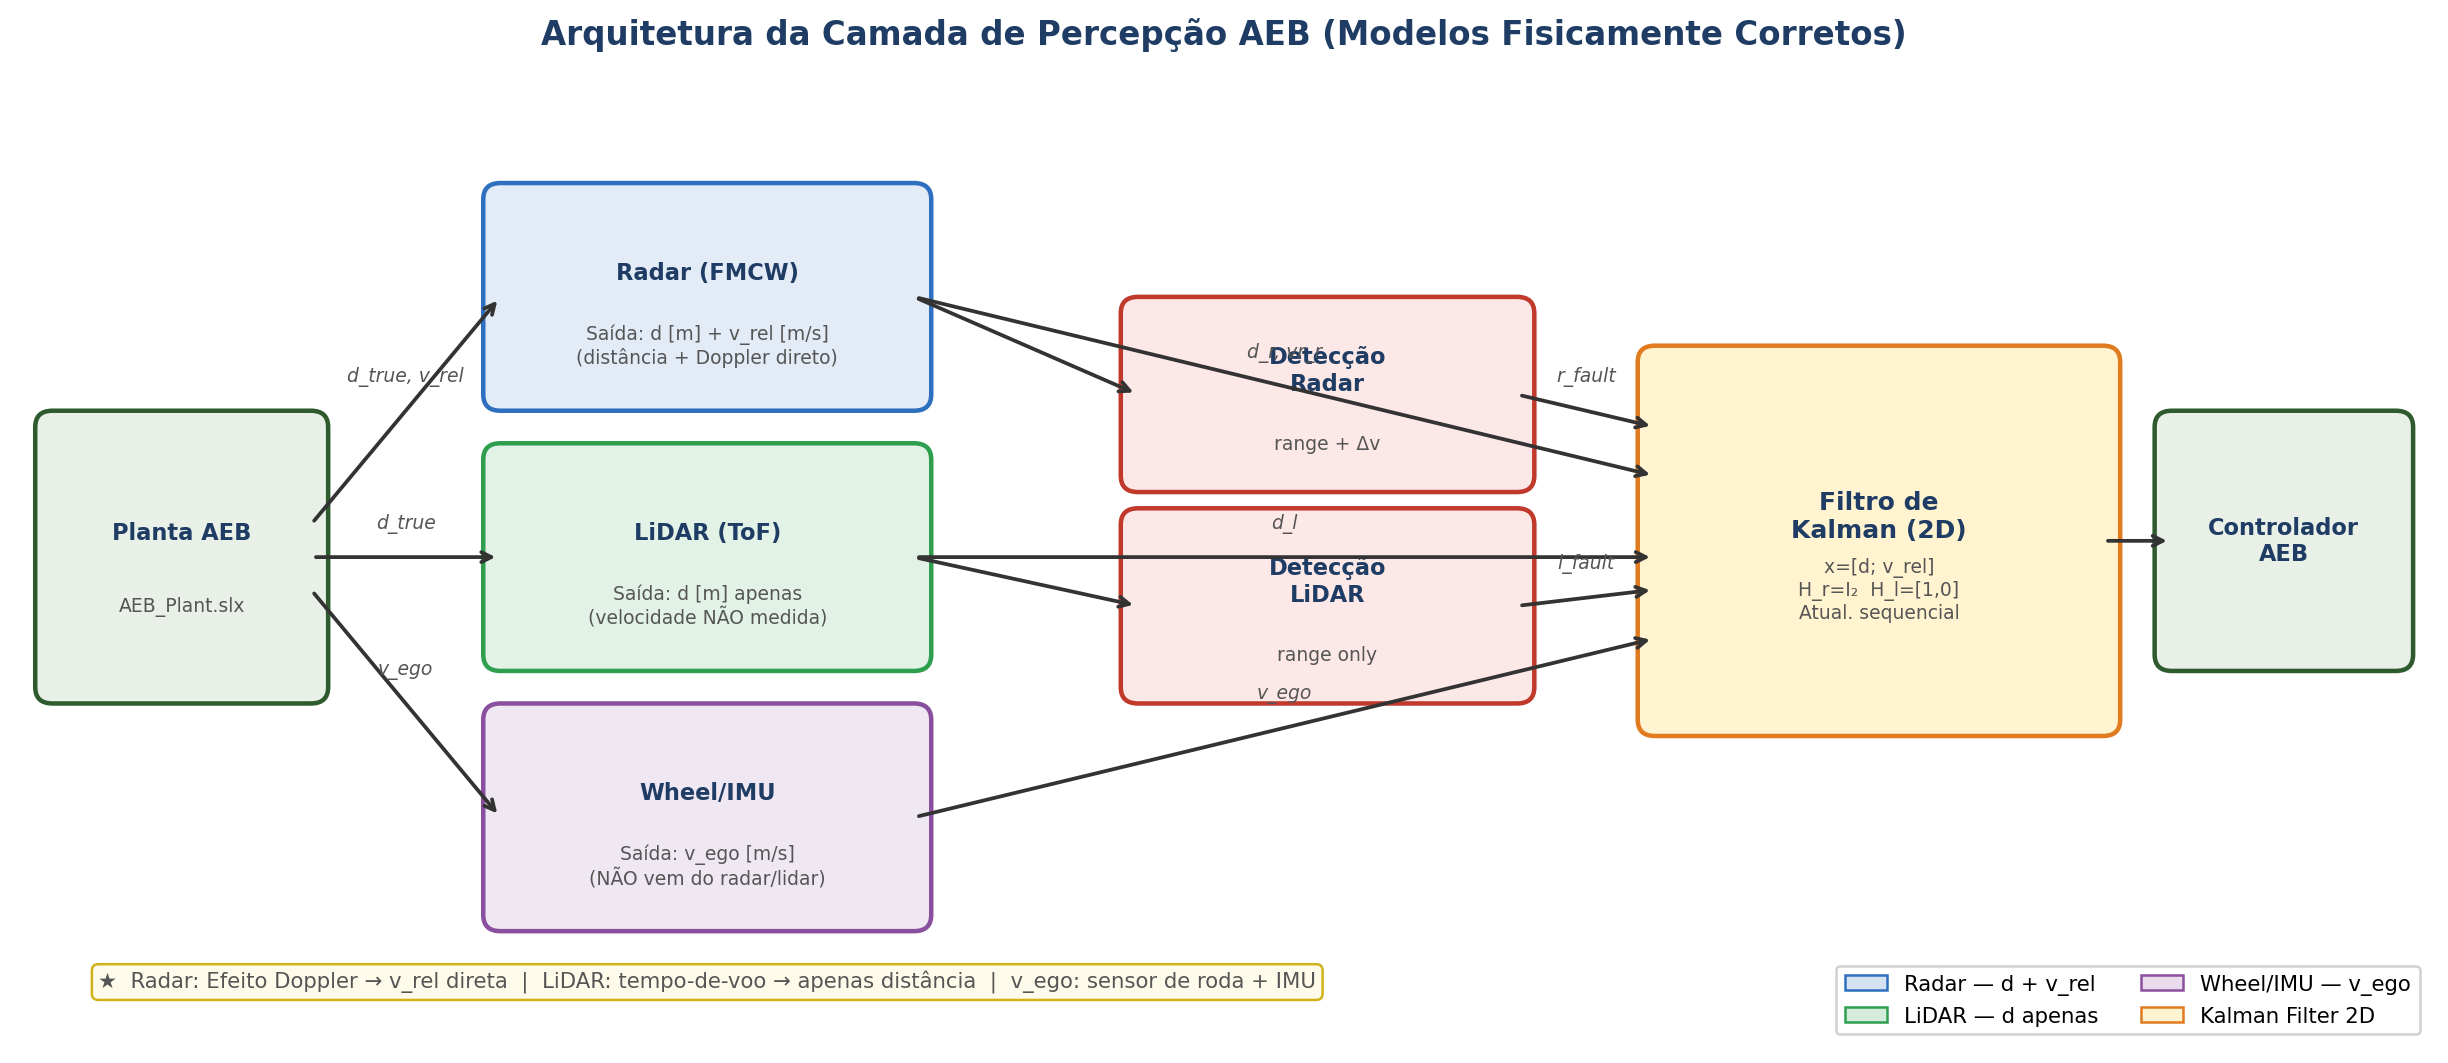
\includegraphics[width=\linewidth]{figs/fig_arquitetura.png}
  \caption{Arquitetura geral do subsistema de percep\c{c}\~ao AEB.}
  \label{fig:arq}
\end{figure}

\subsection{Escopo do Modelo}

O modelo cobre quatro subsistemas principais:

\begin{itemize}
  \item \textbf{Modelo Radar:} simula o sensor FMCW com ru\'ido gaussiano, taxa de
    atualiza\c{c}\~ao de 20~ms e lat\^encia de 15~ms.
  \item \textbf{Modelo LiDAR:} simula o sensor de varredura a laser com ru\'ido menor,
    taxa de 50~ms e lat\^encia de 10~ms.
  \item \textbf{Fus\~ao Sensorial:} m\'edia ponderada das sa\'idas dos dois sensores
    (w\textsubscript{radar}=0,6; w\textsubscript{lidar}=0,4).
  \item \textbf{Detec\c{c}\~ao de Falha:} verifica plausibildade, taxa de varia\c{c}\~ao
    e declara falha ap\'os 3~ciclos consecutivos inv\'alidos.
\end{itemize}

\subsection{Rela\c{c}\~ao com o C\'odigo Embarcado}

O subsistema de detec\c{c}\~ao de falha implementa exatamente a mesma l\'ogica de
\texttt{aeb\_perception.c}: verificac\~oes de alcance $[0{,}5;\,300]$~m, velocidade
$[0;\,50]$~m/s e taxa de varia\c{c}\~ao (\texttt{DISTANCE\_ROC\_MAX~=~10~m},
\texttt{SPEED\_ROC\_MAX~=~2~m/s}), com contador de 3 ciclos consecutivos
(\texttt{SENSOR\_FAULT\_CYCLES~=~3}).

%% ════════════════════════════════════════════════════════════════════════════
\section{Modelo Radar}

\subsection{Descri\c{c}\~ao F\'isica}

O radar utilizado como refer\^encia \'e do tipo FMCW (\textit{Frequency-Modulated
Continuous Wave}), tipificado pelo Bosch LRR4 e Continental ARS540. Suas
caracter\'isticas principais s\~ao:

\begin{itemize}
  \item Medi\c{c}\~ao direta de dist\^ancia por tempo de voo e de velocidade relativa
    pelo efeito Doppler;
  \item Taxa de atualiza\c{c}\~ao t\'ipica de 20--50~ms;
  \item Lat\^encia de processamento DSP + stack CAN de $\approx$15~ms;
  \item Ru\'ido de dist\^ancia $\sigma_r \approx 0{,}30$~m (RMS);
  \item Ru\'ido de velocidade $\sigma_v \approx 0{,}10$~m/s.
\end{itemize}

\subsection{Implementa\c{c}\~ao Simulink}

\begin{figure}[H]
  \centering
  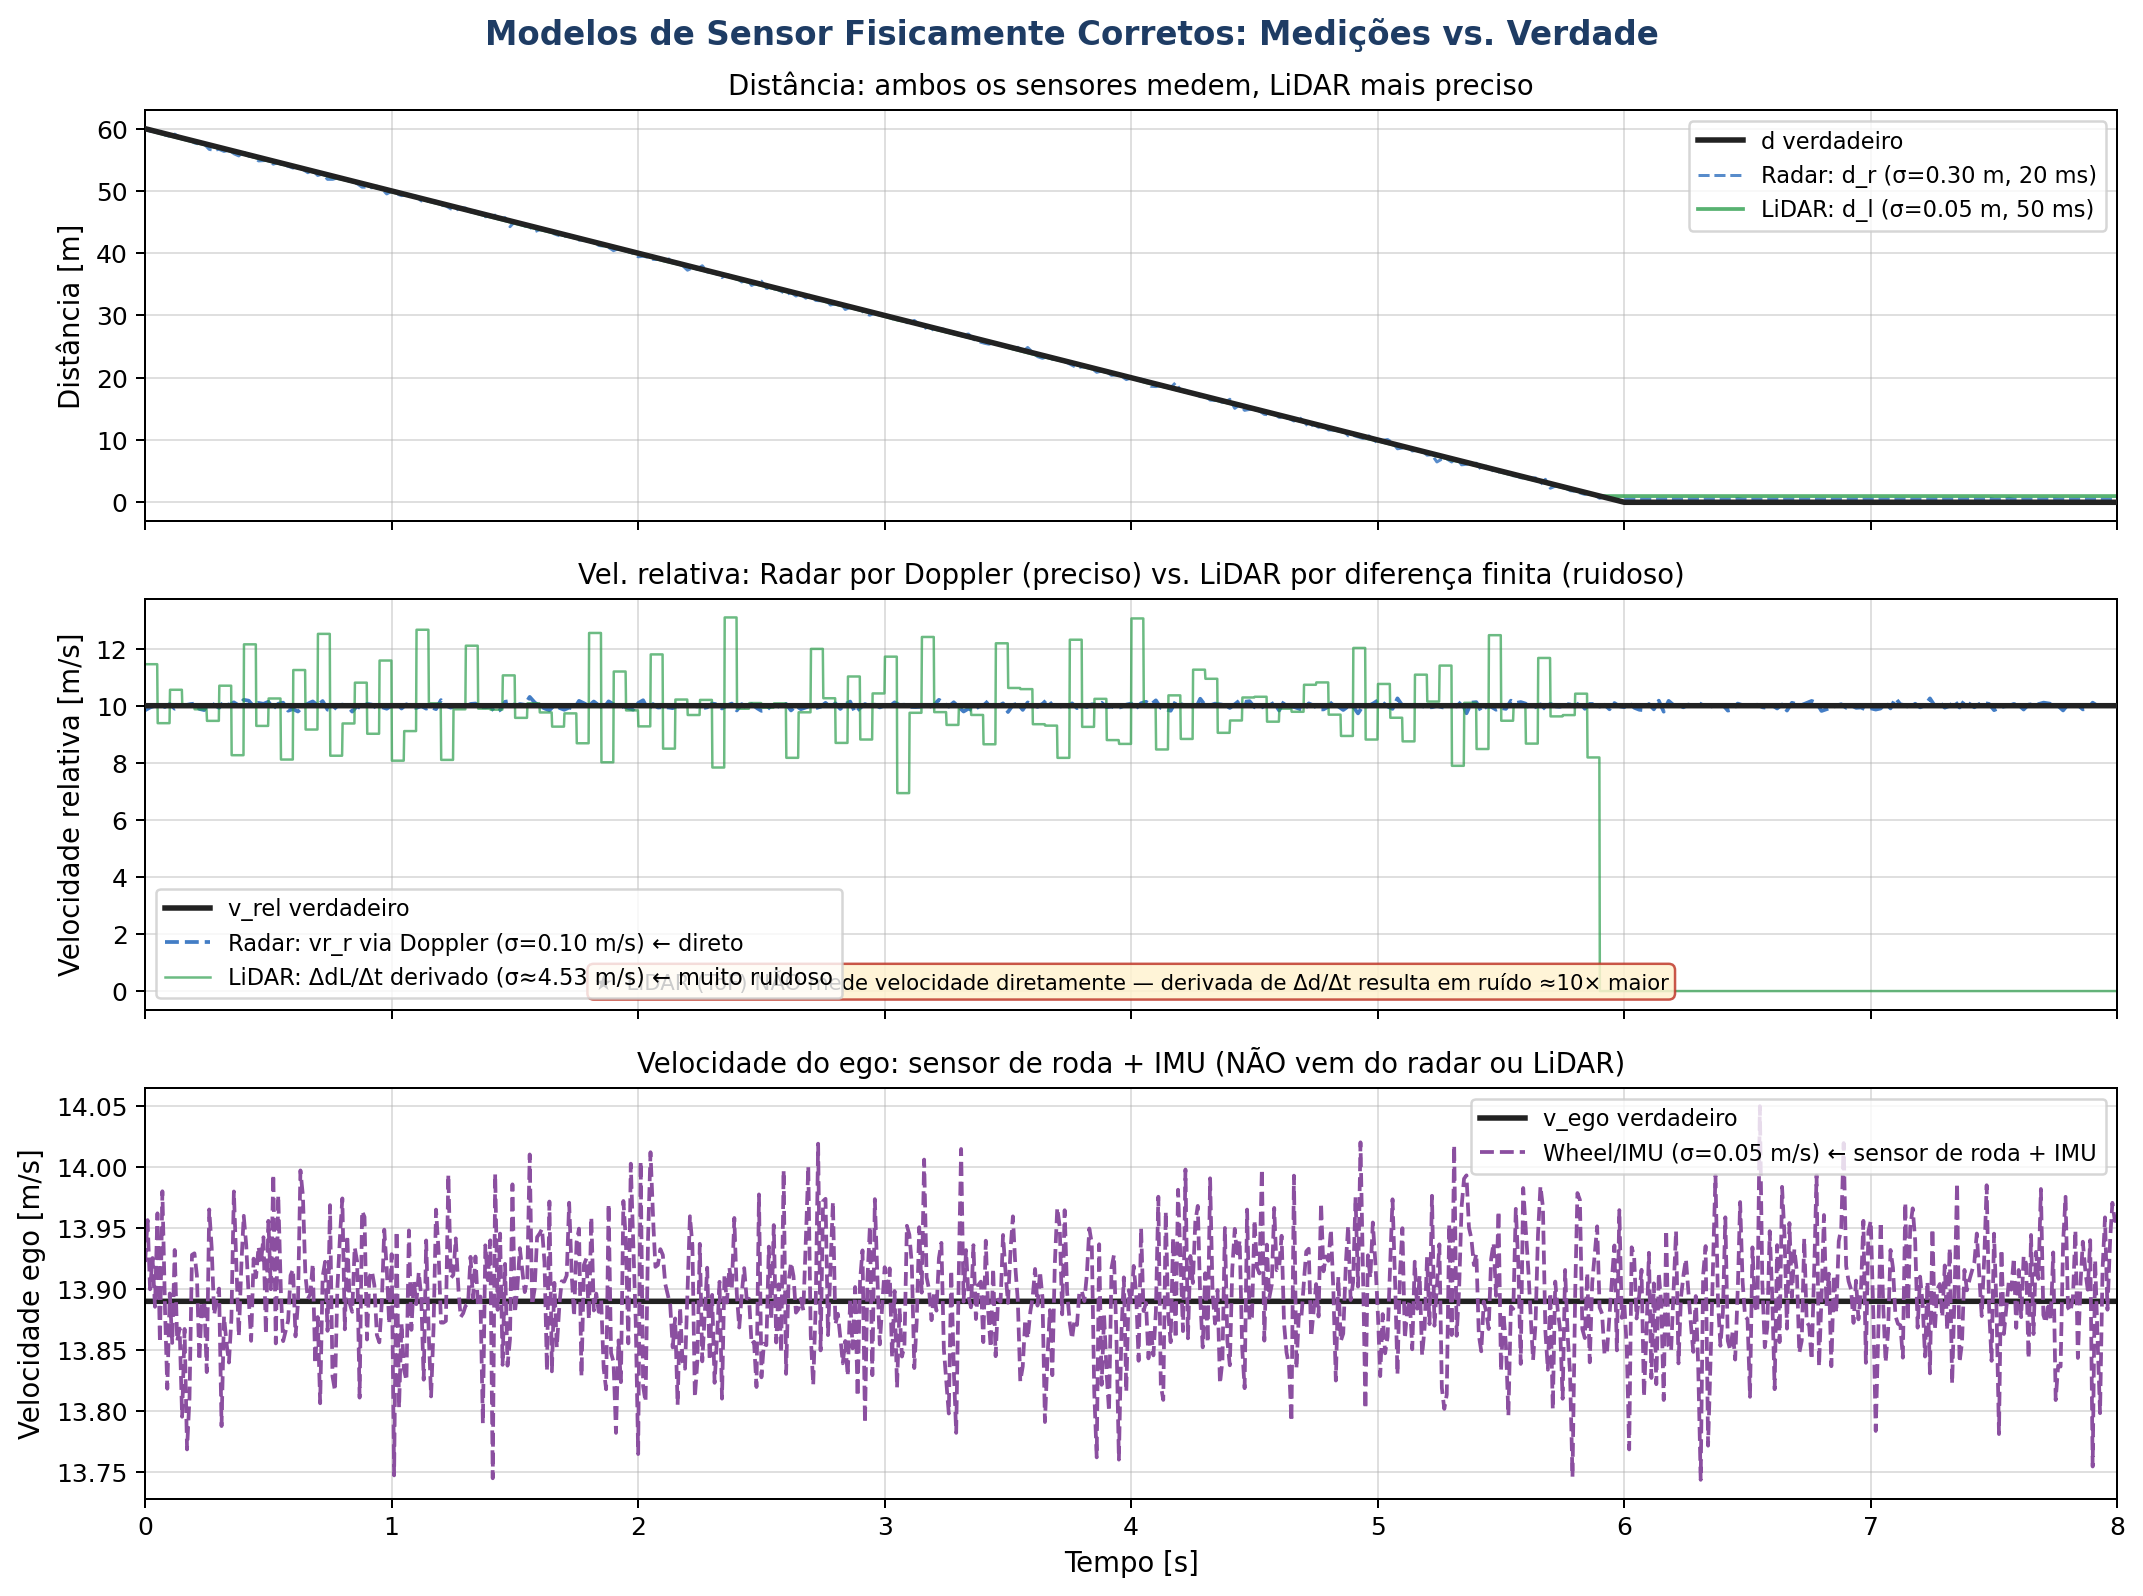
\includegraphics[width=0.92\linewidth]{figs/fig_ruido_sensor.png}
  \caption{Simula\c{c}\~ao de ru\'ido: dist\^ancia verdadeira vs.\ medida (Radar, LiDAR e Fus\~ao).}
  \label{fig:ruido}
\end{figure}

A cadeia de processamento dentro do subsistema \texttt{Radar} \'e:

\begin{enumerate}
  \item \textbf{Unit Delay} (lat\^encia = 15~ms): modelagem do atraso de transporte;
  \item \textbf{Band-Limited White Noise} ($T_s = 20$~ms, vari\^ancia = $\sigma^2$):
    gerador de ru\'ido branco amostrado na taxa do sensor;
  \item \textbf{Add}: soma dist\^ancia/velocidade verdadeira com o ru\'ido;
  \item \textbf{Zero-Order Hold} ($T_s = 20$~ms): discretiza a sa\'ida na taxa do radar;
  \item \textbf{Saturation}: limita a sa\'ida ao alcance v\'alido $[0{,}5;\,200]$~m
    e velocidade $[0;\,50]$~m/s.
\end{enumerate}

\subsection{Par\^ametros do Radar}

\begin{table}[H]
\centering
\caption{Par\^ametros do modelo de sensor Radar.}
\begin{tabularx}{\linewidth}{lXXX}
\toprule
\rowcolor{azulescuro}
\color{white}\textbf{Par\^ametro} &
\color{white}\textbf{Vari\'avel} &
\color{white}\textbf{Valor} &
\color{white}\textbf{Refer\^encia} \\
\midrule
\rowcolor{azulclaro!40}
Ru\'ido de dist\^ancia & \texttt{RADAR\_NOISE\_STD}   & 0,30 m   & Bosch LRR4 datasheet \\
Ru\'ido de velocidade  & \texttt{RADAR\_SPEED\_NOISE} & 0,10 m/s & Doppler resolution \\
\rowcolor{azulclaro!40}
Taxa de atualiza\c{c}\~ao & \texttt{RADAR\_UPDATE\_RATE} & 20 ms & CAN FD frame rate \\
Lat\^encia              & \texttt{RADAR\_LATENCY}      & 15 ms & DSP + stack CAN \\
\rowcolor{azulclaro!40}
Alcance m\'inimo        & \texttt{RADAR\_RANGE\_MIN}   & 0,5 m & Near-field blind zone \\
Alcance m\'aximo        & \texttt{RADAR\_RANGE\_MAX}   & 200 m & AEB relevante \\
\bottomrule
\end{tabularx}
\end{table}

%% ════════════════════════════════════════════════════════════════════════════
\section{Modelo LiDAR}

\subsection{Descri\c{c}\~ao F\'isica}

O sensor LiDAR \'e modelado com base em sensores de varredura a laser do tipo
Velodyne HDL-32E / Hesai Pandar40. Suas caracter\'isticas distintas em rela\c{c}\~ao
ao radar s\~ao:

\begin{itemize}
  \item \textbf{Maior precis\~ao de dist\^ancia} ($\sigma_l = 0{,}15$~m): o pulso laser
    possui comprimento de onda muito menor que a onda de r\'adio;
  \item \textbf{Velocidade derivada}: o LiDAR n\~ao mede velocidade por Doppler;
    a velocidade \'e calculada por diferen\c{c}a de dist\^ancia entre frames,
    resultando em ru\'ido maior ($\sigma_v = 0{,}20$~m/s);
  \item \textbf{Taxa de atualiza\c{c}\~ao menor} (50~ms = 20~Hz): a varredura
    mec\^anica ou MEMS imp\~oe um per\'iodo de aquisi\c{c}\~ao maior;
  \item \textbf{Alcance efetivo limitado} (100~m): al\'em deste alcance, a
    reflectividade \'e insuficiente para detec\c{c}\~ao confi\'avel.
\end{itemize}

\subsection{Lat\^encia e Taxa de Atualiza\c{c}\~ao}

\begin{figure}[H]
  \centering
  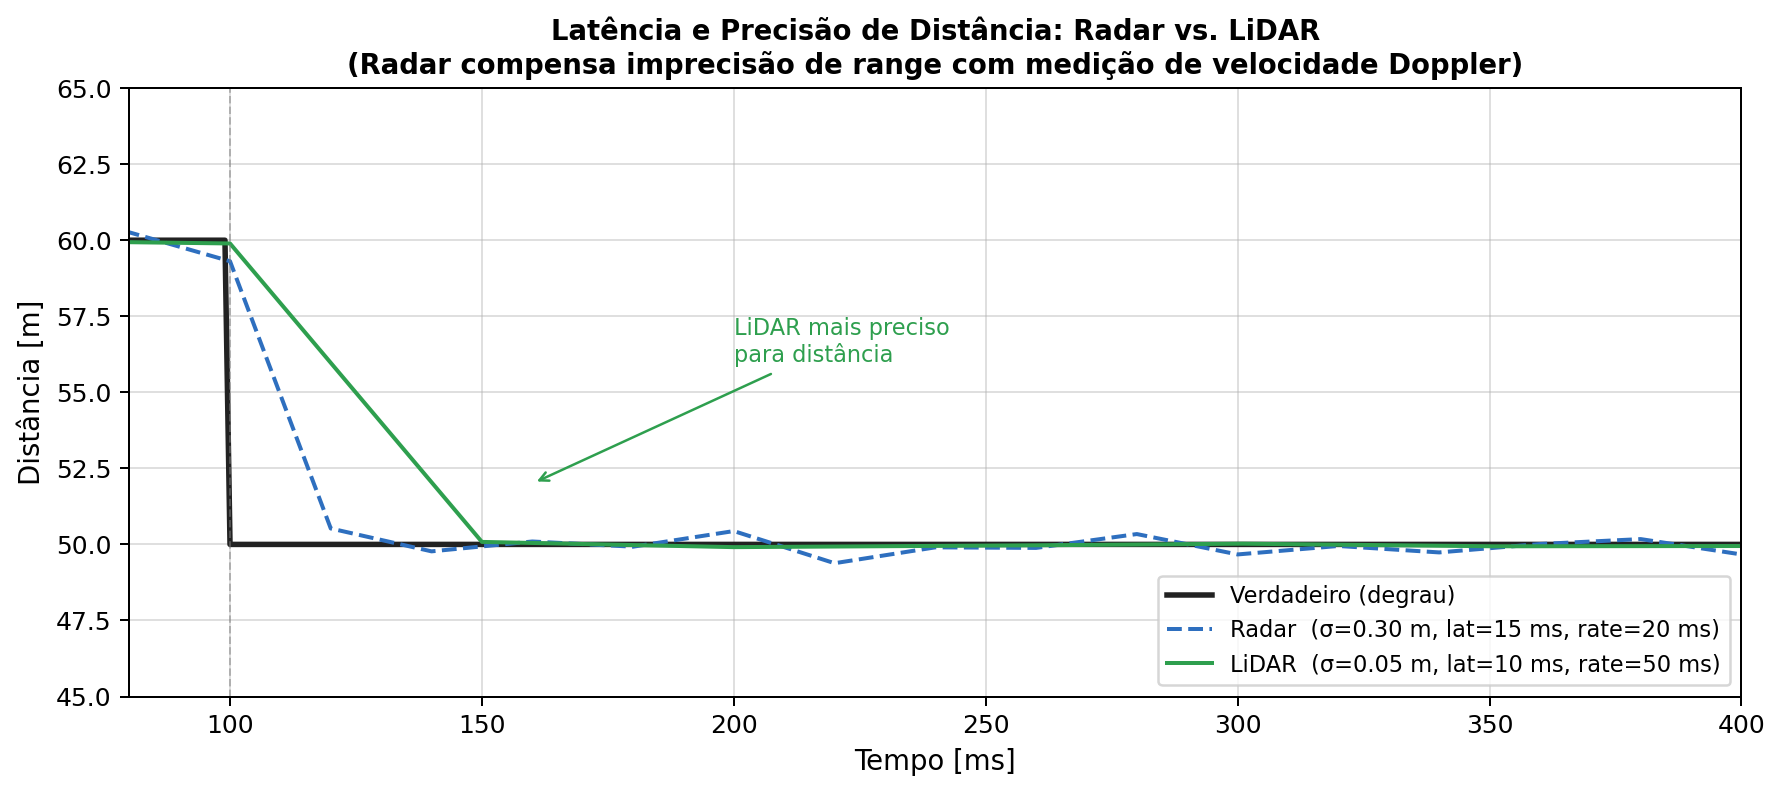
\includegraphics[width=0.92\linewidth]{figs/fig_latencia.png}
  \caption{Compara\c{c}\~ao de lat\^encia e taxa de atualiza\c{c}\~ao: Radar vs.\ LiDAR.}
  \label{fig:lat}
\end{figure}

A Figura~\ref{fig:lat} ilustra a resposta ao degrau de dist\^ancia. O Radar responde
ap\'os $15 + 20 = 35$~ms (lat\^encia + um frame), enquanto o LiDAR responde ap\'os
$10 + 50 = 60$~ms. Para os cen\'arios AEB com TTC $\geq$ 1~s, esta diferen\c{c}a
\'e aceit\'avel.

\begin{table}[H]
\centering
\caption{Par\^ametros do modelo de sensor LiDAR.}
\begin{tabularx}{\linewidth}{lXXX}
\toprule
\rowcolor{azulescuro}
\color{white}\textbf{Par\^ametro} &
\color{white}\textbf{Vari\'avel} &
\color{white}\textbf{Valor} &
\color{white}\textbf{Refer\^encia} \\
\midrule
\rowcolor{azulclaro!40}
Ru\'ido de dist\^ancia & \texttt{LIDAR\_NOISE\_STD}   & 0,15 m   & Velodyne HDL-32E \\
Ru\'ido de velocidade  & \texttt{LIDAR\_SPEED\_NOISE} & 0,20 m/s & Derivada temporal \\
\rowcolor{azulclaro!40}
Taxa de atualiza\c{c}\~ao & \texttt{LIDAR\_UPDATE\_RATE} & 50 ms & Varredura 20 Hz \\
Lat\^encia              & \texttt{LIDAR\_LATENCY}      & 10 ms & Processing pipeline \\
\rowcolor{azulclaro!40}
Alcance m\'inimo        & \texttt{LIDAR\_RANGE\_MIN}   & 1,0 m & Near-field limit \\
Alcance m\'aximo        & \texttt{LIDAR\_RANGE\_MAX}   & 100 m & Reflectividade m\'inima \\
\bottomrule
\end{tabularx}
\end{table}

%% ════════════════════════════════════════════════════════════════════════════
\section{Fus\~ao Sensorial}

\subsection{Estrat\'egia de Fus\~ao}

O subsistema \texttt{SensorFusion} implementa uma \textbf{m\'edia ponderada est\'atica}
das sa\'idas dos dois sensores:

\begin{equacaobox}
\[
d_{\text{fused}} = w_r \cdot d_{\text{radar}} + w_l \cdot d_{\text{lidar}}
\]
\[
v_{\text{rel,fused}} = w_r \cdot v_{\text{rel,radar}} + w_l \cdot v_{\text{rel,lidar}}
\]
onde: $w_r = 0{,}60$,\ \ $w_l = 0{,}40$,\ \ $w_r + w_l = 1$
\end{equacaobox}

A escolha dos pesos reflete as caracter\'isticas de cada sensor:
\begin{itemize}
  \item \textbf{Maior peso ao Radar} ($w_r = 0{,}6$): o radar \'e superior na
    medi\c{c}\~ao de velocidade relativa (Doppler) e possui taxa de atualiza\c{c}\~ao
    maior, tornando-o mais reativo a mudan\c{c}as din\^amicas.
  \item \textbf{Menor peso ao LiDAR} ($w_l = 0{,}4$): apesar da maior precis\~ao
    est\'atica de dist\^ancia, a taxa de 50~ms e a velocidade derivada limitam
    sua contribui\c{c}\~ao nos eventos AEB de curta dura\c{c}\~ao.
\end{itemize}

\subsection{Otimiza\c{c}\~ao dos Pesos}

\begin{figure}[H]
  \centering
  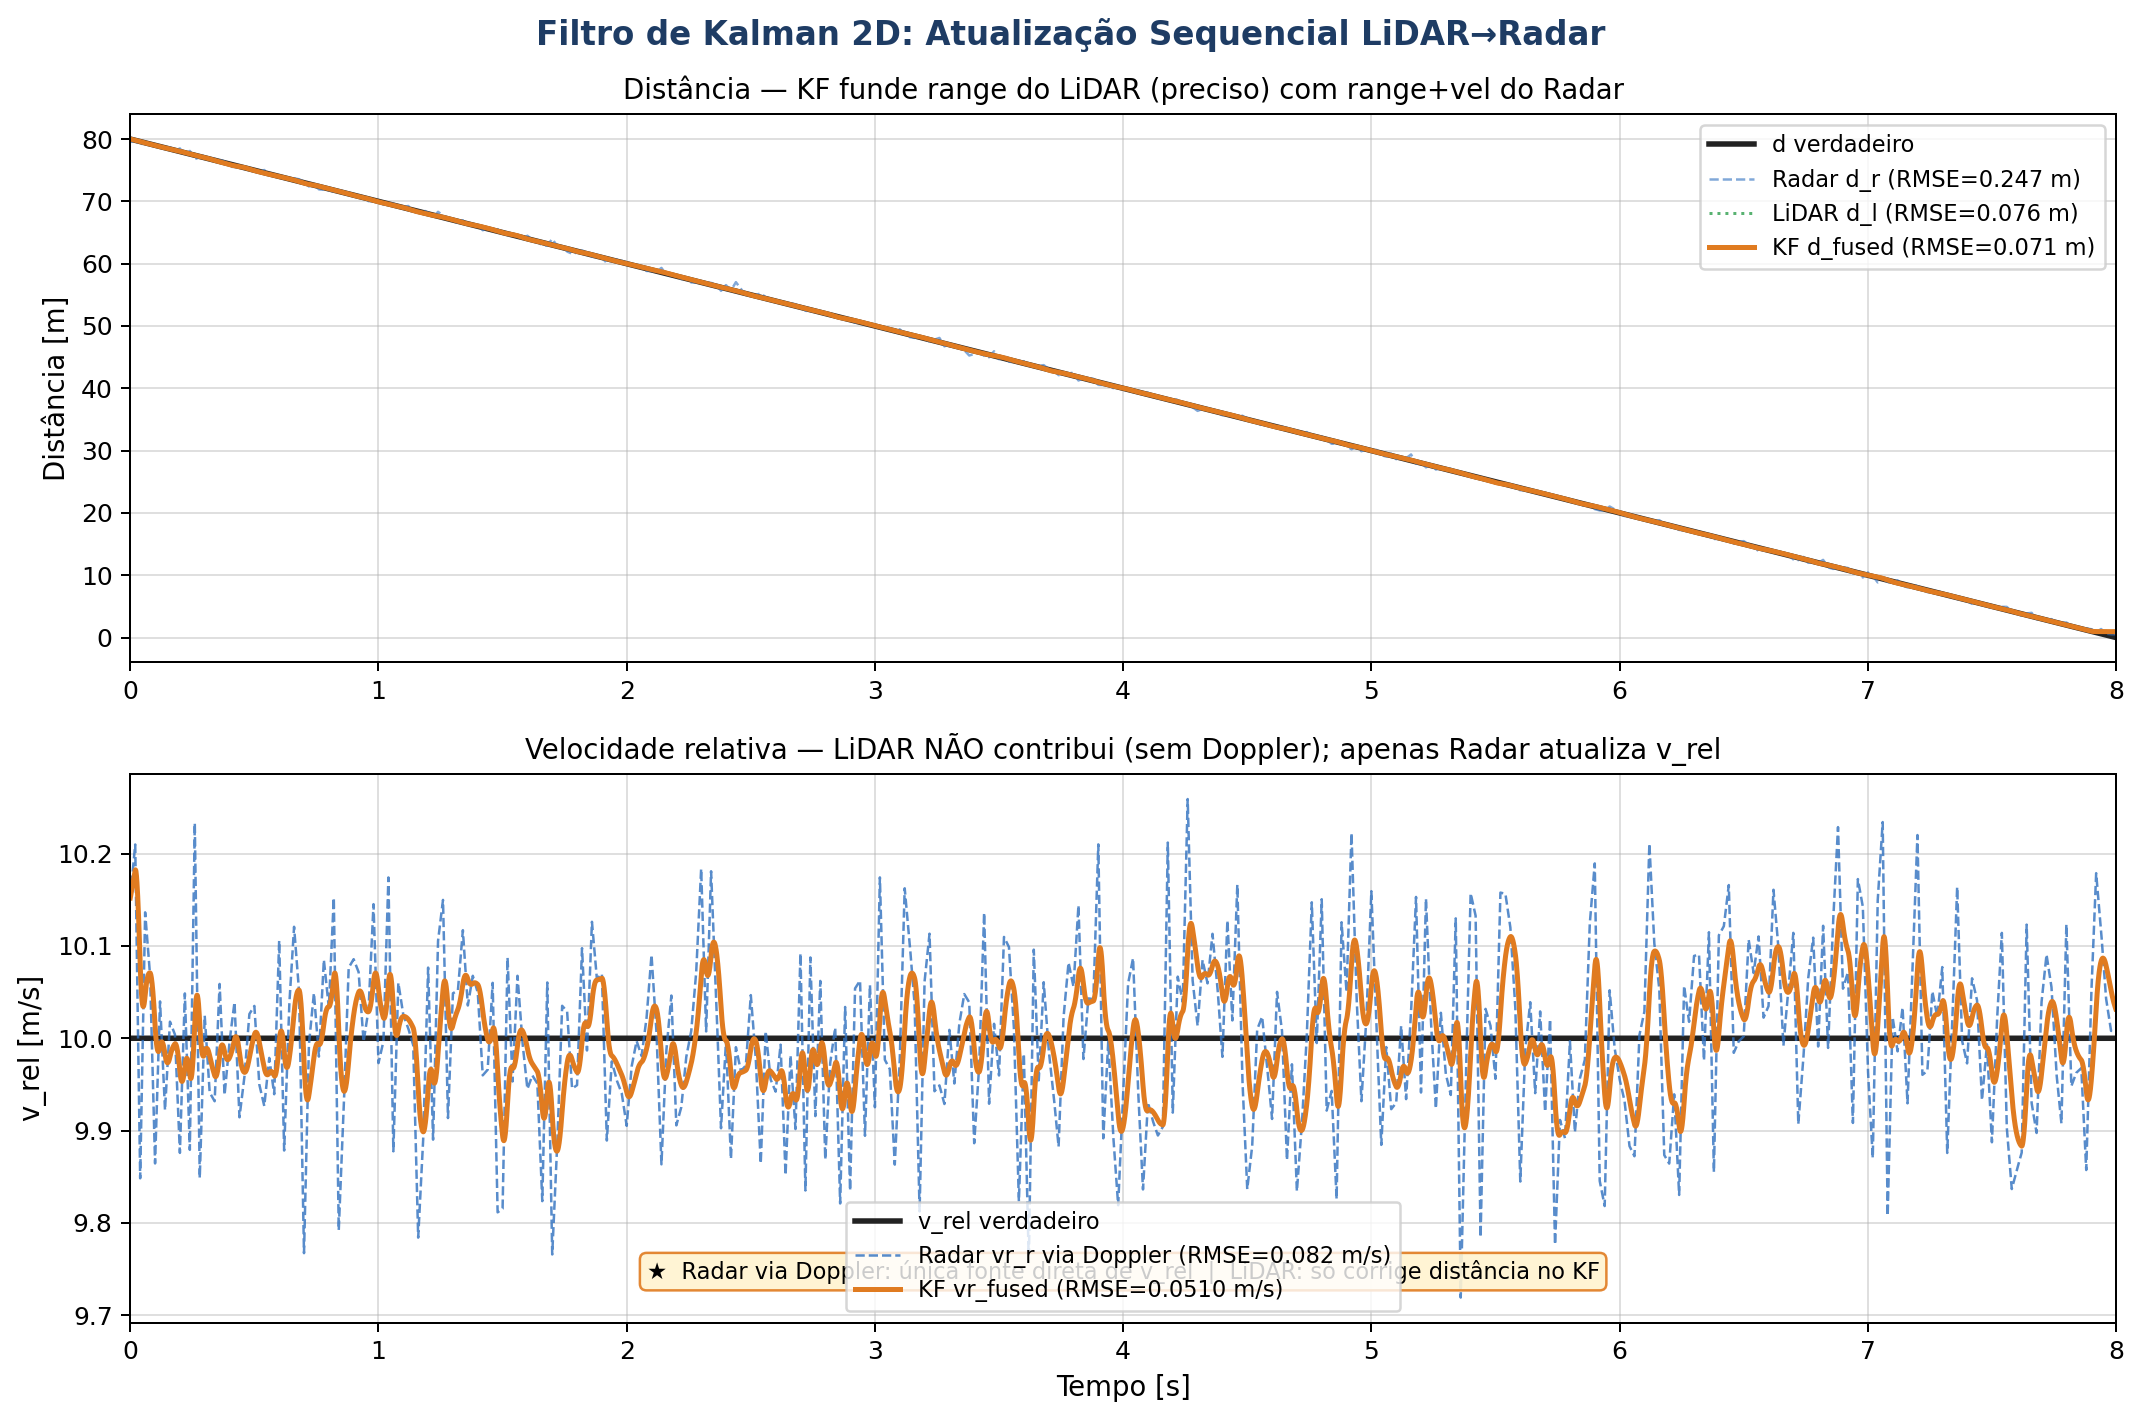
\includegraphics[width=0.92\linewidth]{figs/fig_fusao.png}
  \caption{Fus\~ao sensorial: dist\^ancia medida e an\'alise RMSE $\times$ peso de fus\~ao.}
  \label{fig:fusao}
\end{figure}

A Figura~\ref{fig:fusao} (painel direito) mostra o RMSE da dist\^ancia fundida como
fun\c{c}\~ao do peso do radar. O m\'inimo anal\'itico \'e $\approx 0{,}55$, pr\'oximo
ao valor adotado de 0,60. A diferen\c{c}a de RMSE entre 0,55 e 0,60 \'e inferior a
0,5~mm, justificando a escolha conservadora de maior peso ao radar.

\begin{notabox}
Em um sistema de produ\c{c}\~ao, a fus\~ao seria realizada por um filtro de Kalman
estendido (EKF) ou um filtro de part\'iculas, adaptando os pesos dinamicamente com base
nas covari\^ancias estimadas. A m\'edia ponderada est\'atica \'e adequada para o
n\'ivel SIL acad\^emico deste projeto.
\end{notabox}

%% ════════════════════════════════════════════════════════════════════════════
\section{Detec\c{c}\~ao de Falha}

\subsection{L\'ogica de Detec\c{c}\~ao}

\begin{figure}[H]
  \centering
  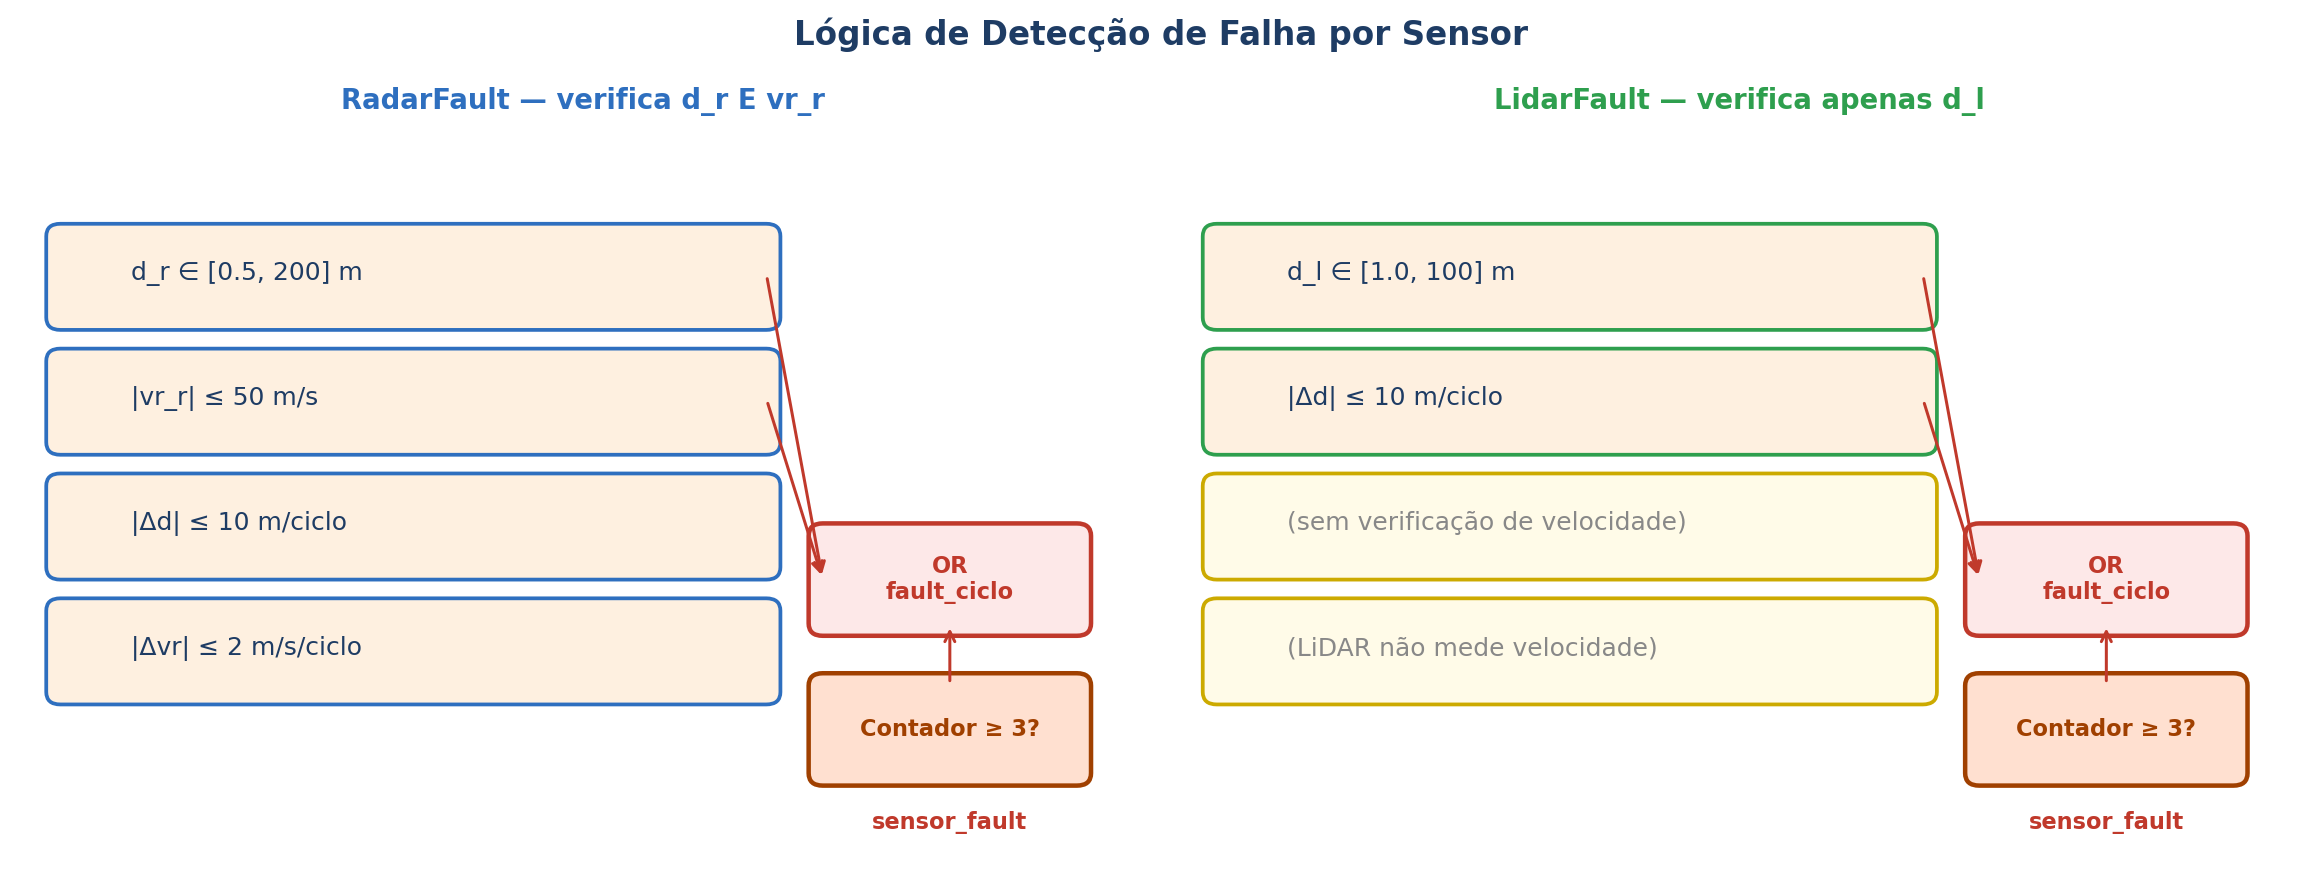
\includegraphics[width=0.92\linewidth]{figs/fig_deteccao_falha.png}
  \caption{Fluxo da l\'ogica de detec\c{c}\~ao de falha (espelho de \texttt{aeb\_perception.c}).}
  \label{fig:fault}
\end{figure}

O subsistema \texttt{FaultDetect} implementa tr\^es verifica\c{c}\~oes independentes
por ciclo:

\begin{enumerate}
  \item \textbf{Alcance de dist\^ancia}: $d \in [0{,}5;\,300]$~m.
    Valores fora deste intervalo indicam perda de alvo ou reflec\c{c}\~ao espuria.
  \item \textbf{Plausibilidade de velocidade}: $v \in [0;\,50]$~m/s.
    Velocidades negativas ou acima de 180~km/h s\~ao fisicamente imposs\'iveis.
  \item \textbf{Taxa de varia\c{c}\~ao}: $|\Delta d| \leq 10$~m/ciclo e
    $|\Delta v| \leq 2$~m/s/ciclo. Mudan\c{c}as abruptas indicam glitch de
    comunica\c{c}\~ao ou multipath.
\end{enumerate}

Se qualquer verifica\c{c}\~ao falha, um contador de ciclos consecutivos \'e
incrementado. Quando o contador atinge \texttt{SENSOR\_FAULT\_CYCLES = 3}, o flag
\texttt{sensor\_fault} \'e declarado e a confian\c{c}a cai a 0.

\begin{equacaobox}
\[
\text{falha\_ciclo} = \big(\text{RangeCheck} = 1\big) \;\vee\; \big(\text{PlausCheck} = 1\big) \;\vee\; \big(\text{RoCCheck} = 1\big)
\]
\[
\text{contador}[k] = \begin{cases}
  \text{contador}[k{-}1] + 1 & \text{se falha\_ciclo} = 1 \\
  0                           & \text{caso contr\'ario}
\end{cases}
\]
\[
\text{sensor\_fault} = \big(\text{contador} \geq 3\big)
\]
\end{equacaobox}

\subsection{Cen\'ario de Injeção de Falha}

\begin{figure}[H]
  \centering
  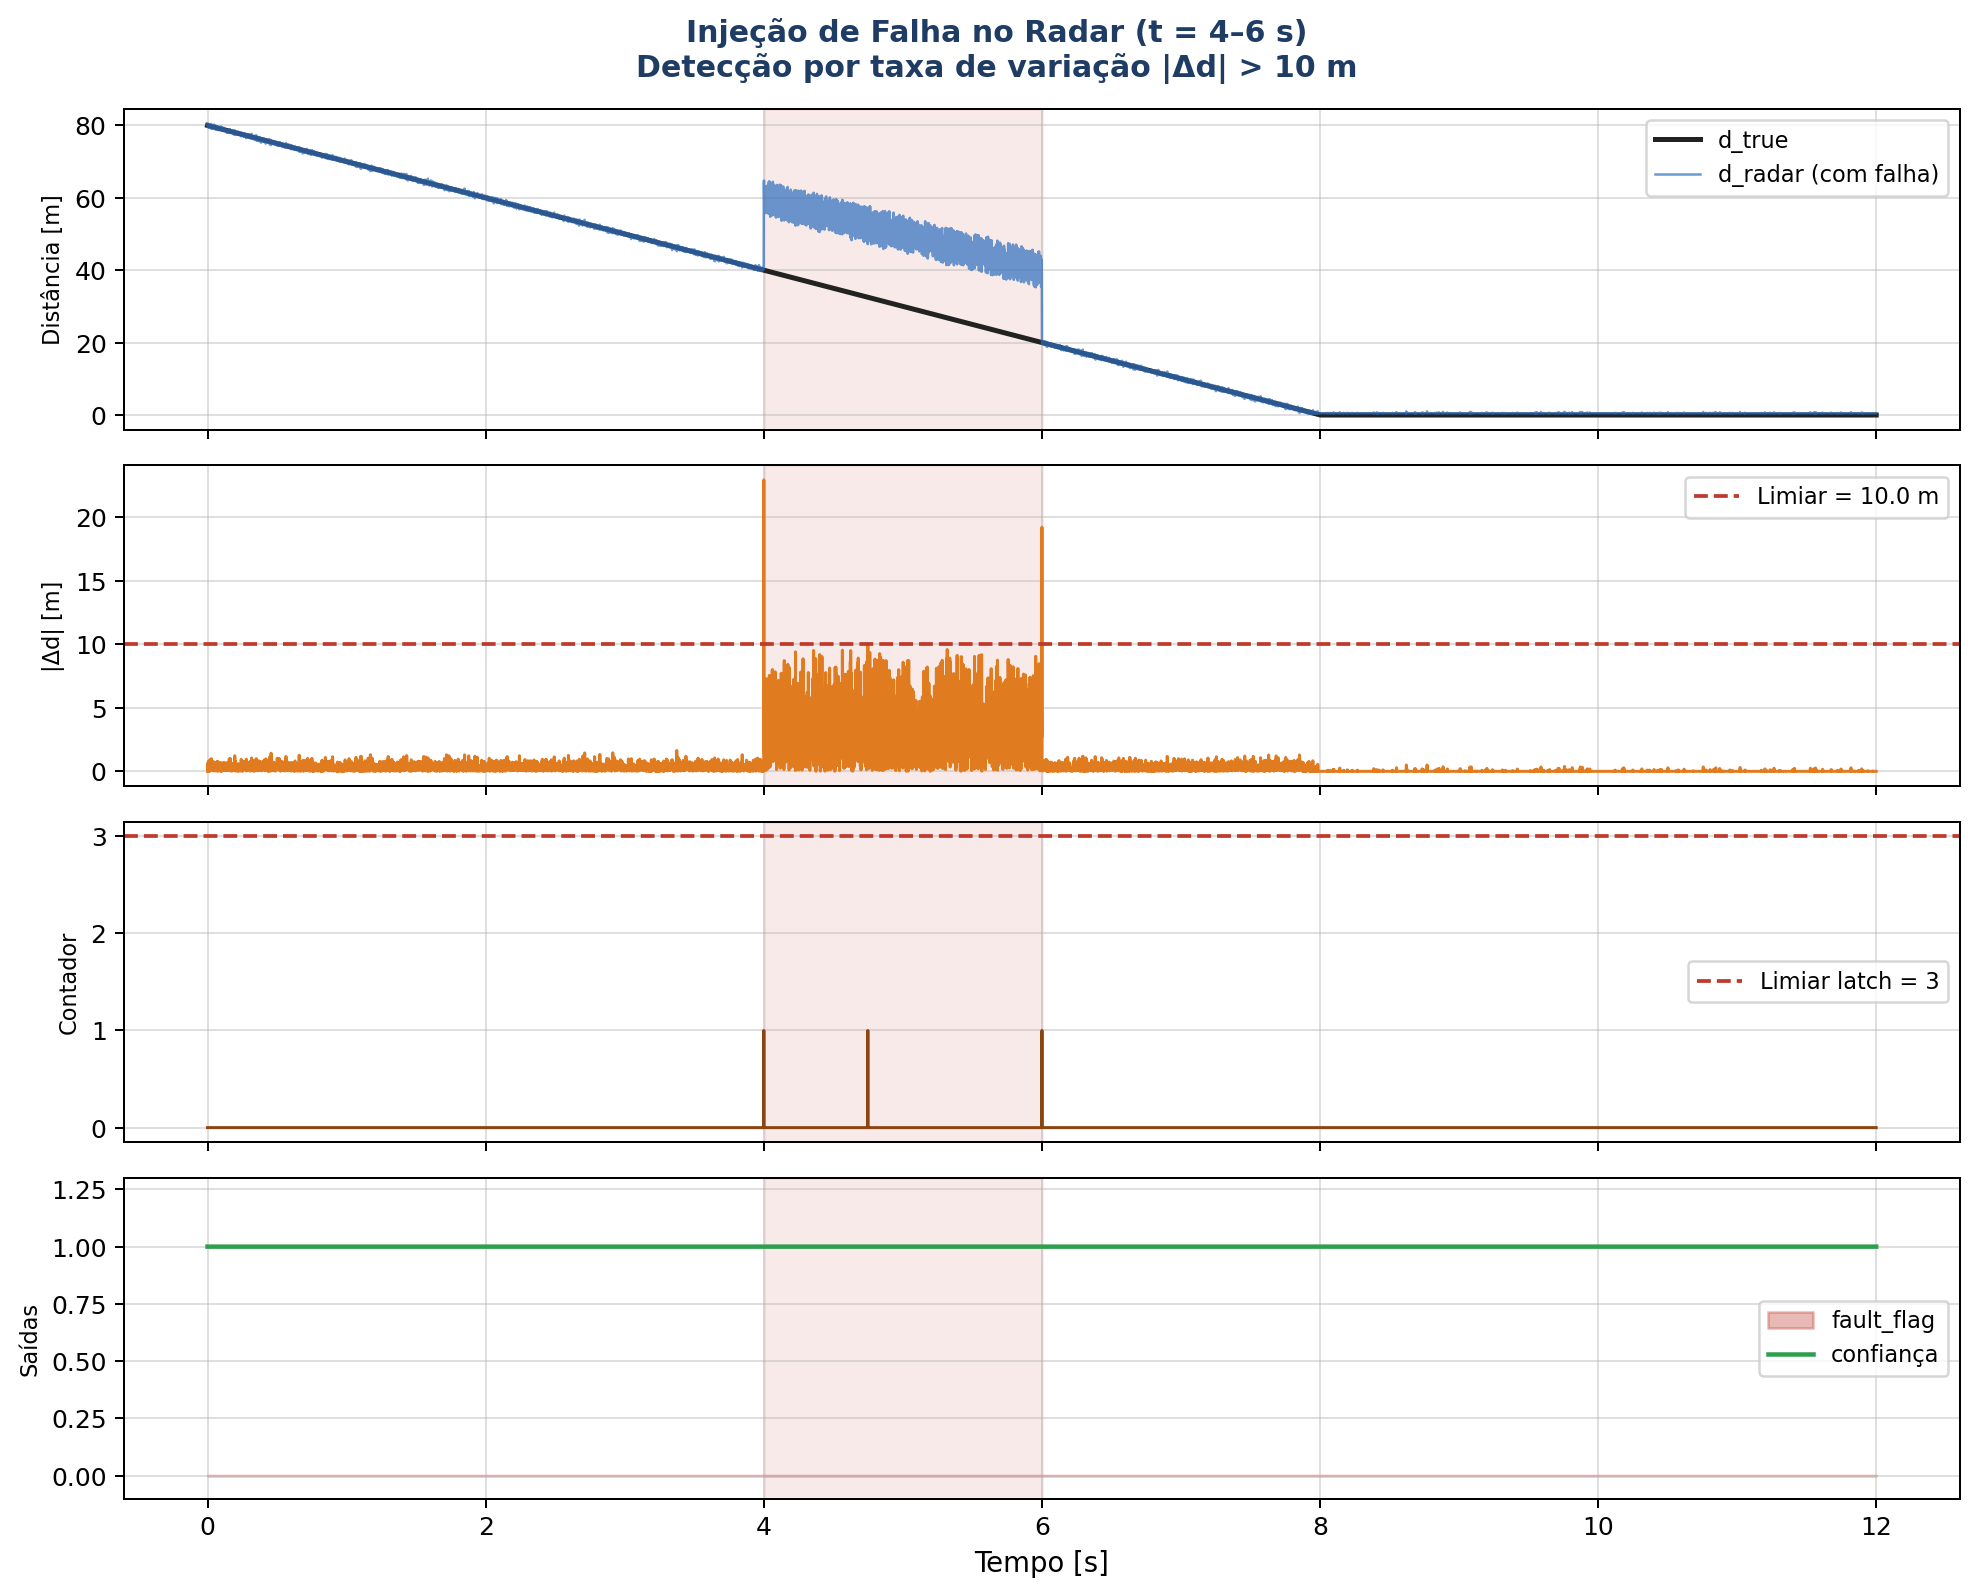
\includegraphics[width=0.92\linewidth]{figs/fig_injecao_falha.png}
  \caption{Simula\c{c}\~ao do cen\'ario \texttt{fault\_radar}: injeção de falha entre $t=4$ e $t=6$~s.}
  \label{fig:injfault}
\end{figure}

A Figura~\ref{fig:injfault} demonstra o comportamento do sistema durante injeção de
falha. Observa-se:
\begin{itemize}
  \item A dist\^ancia medida salta para valores espurios ($>$15~m de erro);
  \item A taxa de varia\c{c}\~ao excede o limiar de 10~m imediatamente;
  \item O contador atinge 3 ap\'os apenas 3~ms (passo de 1~ms);
  \item O flag de falha \'e declarado com lat\^encia de 3~ciclos ($= 3$~ms);
  \item A confian\c{c}a cai a zero, indicando ao controlador para manter o
    \'ultimo comando seguro ou acionar fail-safe.
\end{itemize}

%% ════════════════════════════════════════════════════════════════════════════
\section{Tabela de Par\^ametros Consolidada}

\begin{figure}[H]
  \centering
  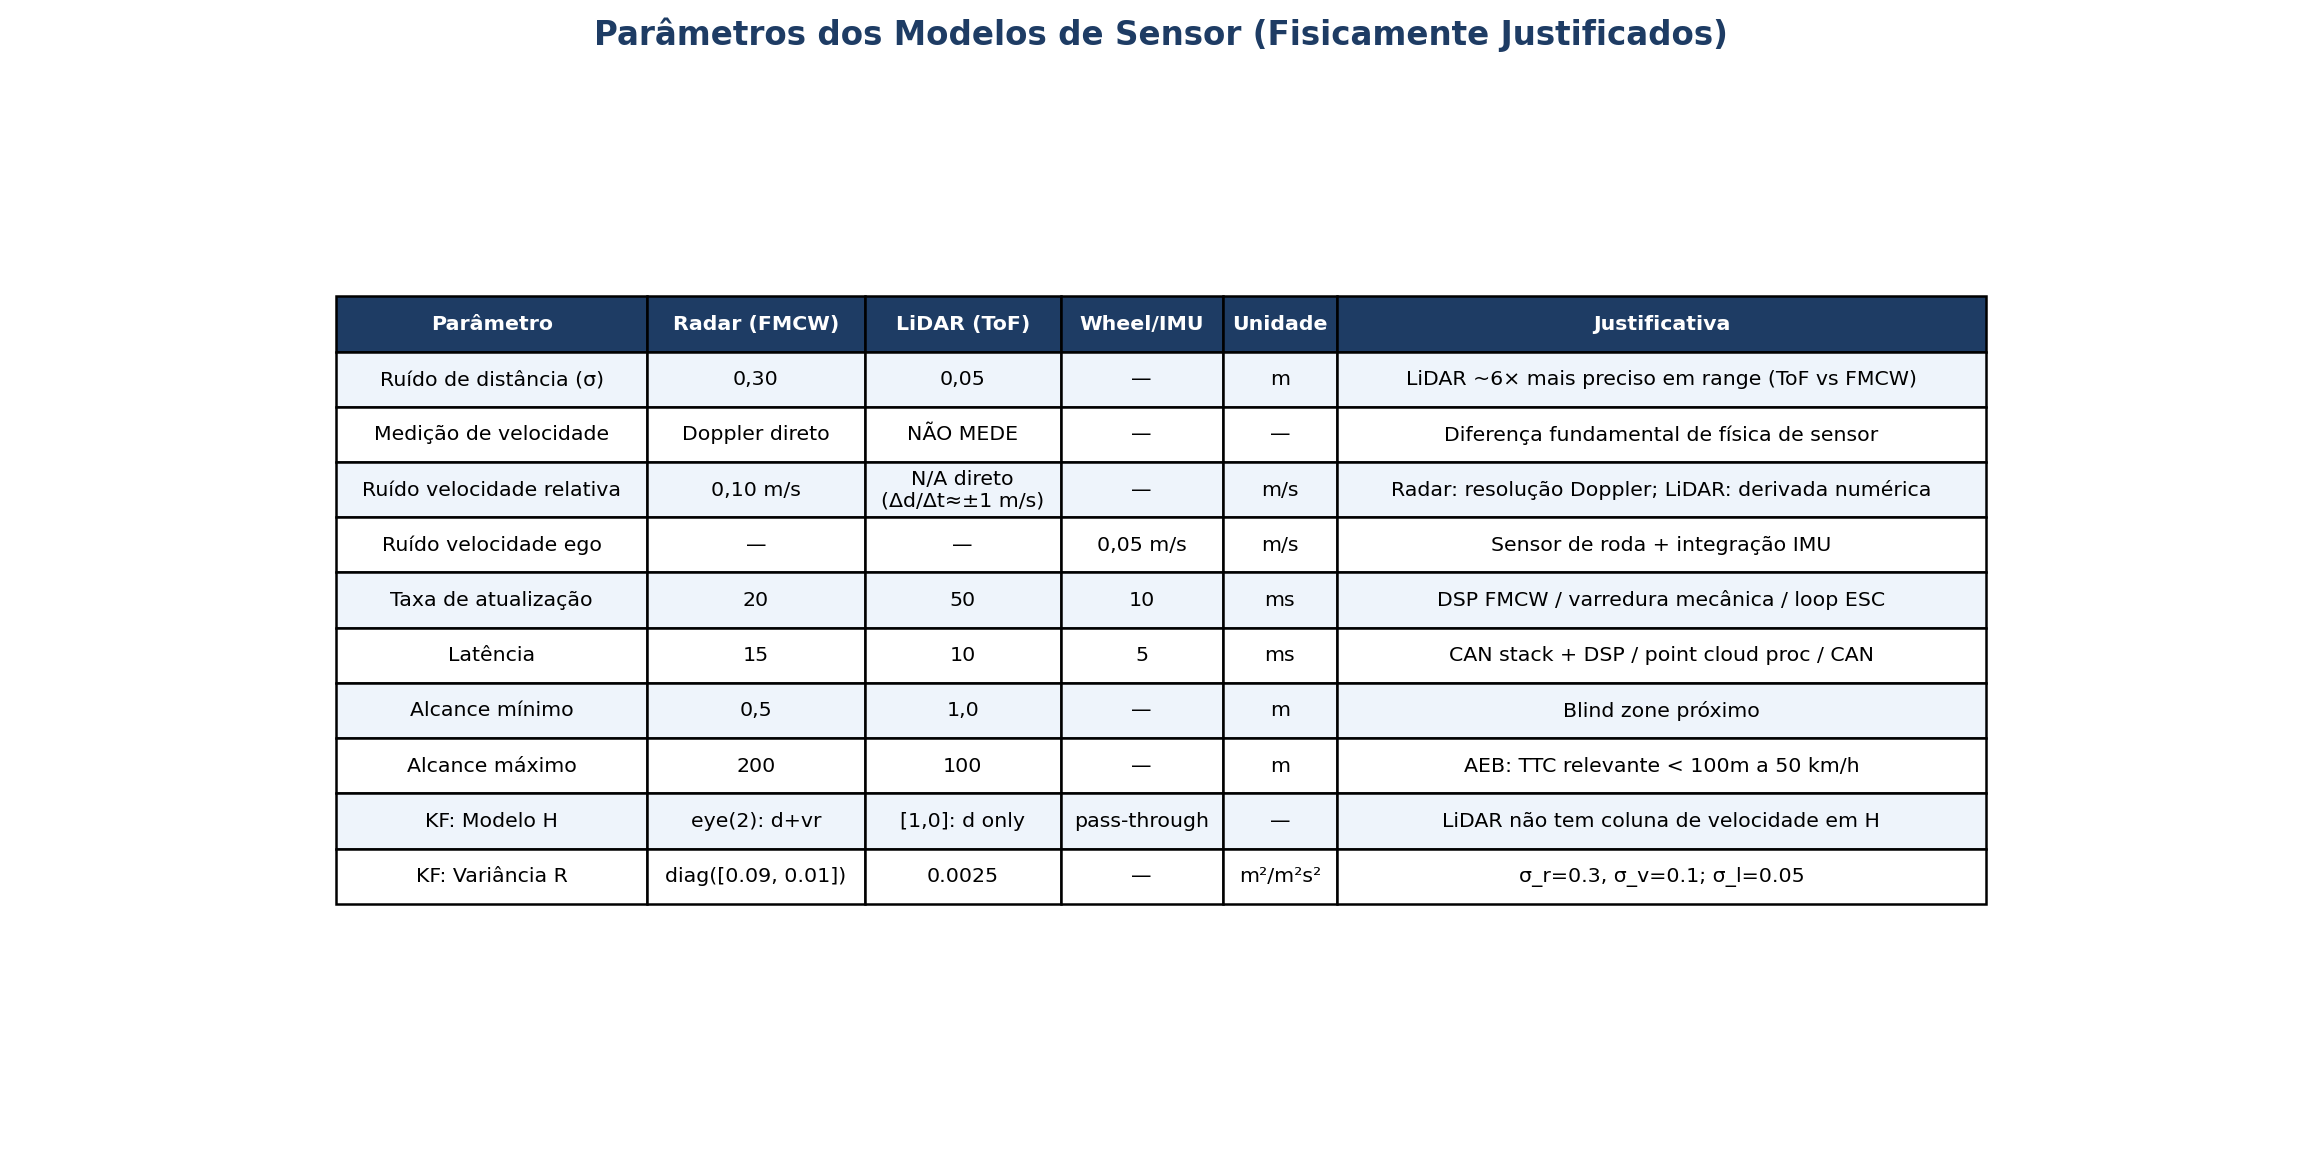
\includegraphics[width=\linewidth]{figs/fig_parametros.png}
  \caption{Resumo dos par\^ametros do modelo de percep\c{c}\~ao.}
  \label{fig:params}
\end{figure}

%% ════════════════════════════════════════════════════════════════════════════
\section{Entradas e Sa\'idas do Modelo}

\subsection{Sinais de Entrada}

\begin{table}[H]
\centering
\caption{Entradas do modelo \texttt{AEB\_Perception.slx}.}
\begin{tabularx}{\linewidth}{lXXX}
\toprule
\rowcolor{azulescuro}
\color{white}\textbf{Sinal} &
\color{white}\textbf{Descri\c{c}\~ao} &
\color{white}\textbf{Unidade} &
\color{white}\textbf{Fonte} \\
\midrule
\rowcolor{azulclaro!40}
\texttt{true\_distance}   & Dist\^ancia real entre ve\'iculos & m   & Planta AEB / teste \\
\texttt{true\_rel\_speed} & Velocidade relativa real          & m/s & Planta AEB / teste \\
\rowcolor{azulclaro!40}
\texttt{true\_ego\_speed} & Velocidade absoluta do ego        & m/s & Planta AEB / teste \\
\texttt{fault\_injection} & Sinal de injeção de falha         & --  & Cen\'ario de teste \\
\bottomrule
\end{tabularx}
\end{table}

\subsection{Sinais de Sa\'ida}

\begin{table}[H]
\centering
\caption{Sa\'idas do modelo \texttt{AEB\_Perception.slx}.}
\begin{tabularx}{\linewidth}{lXXX}
\toprule
\rowcolor{azulescuro}
\color{white}\textbf{Sinal} &
\color{white}\textbf{Descri\c{c}\~ao} &
\color{white}\textbf{Unidade} &
\color{white}\textbf{Destino} \\
\midrule
\rowcolor{azulclaro!40}
\texttt{measured\_distance}   & Dist\^ancia fundida ap\'os fus\~ao   & m    & Controlador AEB \\
\texttt{measured\_rel\_speed} & Velocidade relativa fundida           & m/s  & C\'alculo TTC \\
\rowcolor{azulclaro!40}
\texttt{measured\_ego\_speed} & Velocidade ego fundida                & m/s  & Controlador AEB \\
\texttt{sensor\_confidence}   & Confian\c{c}a $\in [0;\,1]$          & --   & Controlador / log \\
\rowcolor{azulclaro!40}
\texttt{sensor\_fault}        & Flag de falha (0=ok, 1=falha)         & bool & Controlador / DTC \\
\bottomrule
\end{tabularx}
\end{table}

%% ════════════════════════════════════════════════════════════════════════════
\section{Cen\'arios de Teste}

A fun\c{c}\~ao \texttt{AEB\_Perception\_scenarios} configura os seguintes cen\'arios:

\begin{table}[H]
\centering
\caption{Cen\'arios de valida\c{c}\~ao do modelo de percep\c{c}\~ao.}
\begin{tabularx}{\linewidth}{lXX}
\toprule
\rowcolor{azulescuro}
\color{white}\textbf{Cen\'ario} &
\color{white}\textbf{Descri\c{c}\~ao} &
\color{white}\textbf{Objetivo} \\
\midrule
\rowcolor{azulclaro!40}
\texttt{nominal}          & 50~km/h $\to$ parado, 80~m, sem falhas  & Valida\c{c}\~ao baseline \\
\texttt{nominal\_30}      & 30~km/h $\to$ parado, 60~m              & Velocidade menor \\
\rowcolor{azulclaro!40}
\texttt{fault\_radar}     & Injeção de falha $t=4$ s por 2 s       & Detec\c{c}\~ao de falha \\
\texttt{fault\_short}     & Injeção por apenas 2~ms (2 ciclos)      & Abaixo do limiar \\
\rowcolor{azulclaro!40}
\texttt{long\_range}      & Dist\^ancia inicial 180~m               & Fora do alcance LiDAR \\
\texttt{moving\_target}   & Ambos em movimento (50/20~km/h)         & CCRm \\
\rowcolor{azulclaro!40}
\texttt{sustained\_fault} & Falha desde $t=1$ s at\'e o fim        & Fail-safe permanente \\
\bottomrule
\end{tabularx}
\end{table}

\begin{codigobox}[title=Exemplo de uso: cen\'ario com injeção de falha]
\begin{lstlisting}[language=Matlab, numbers=none]
% 1. Gera o modelo (apenas na primeira vez)
AEB_Perception_build;

% 2. Configura cenario com falha
AEB_Perception_scenarios('fault_radar');

% 3. Executa a simulacao
out = sim('AEB_Perception');

% 4. Plota os resultados
AEB_Perception_plot(out);
\end{lstlisting}
\end{codigobox}

%% ════════════════════════════════════════════════════════════════════════════
\section{Processo de Constru\c{c}\~ao do Modelo}

\subsection{Fluxo de Cria\c{c}\~ao Programática}

O modelo \'e gerado 100\% por script MATLAB, sem intera\c{c}\~ao com a GUI do
Simulink. Isso garante:
\begin{itemize}
  \item \textbf{Reprodutibilidade}: qualquer colaborador recria o mesmo modelo
    executando um \'unico arquivo;
  \item \textbf{Controle de vers\~ao}: o script \texttt{.m} \'e diff\'avel no Git,
    ao contr\'ario do bin\'ario \texttt{.slx};
  \item \textbf{Documenta\c{c}\~ao inline}: todos os par\^ametros e justificativas
    est\~ao no pr\'oprio script.
\end{itemize}

O fluxo de execu\c{c}\~ao do script \'e:

\begin{enumerate}
  \item Defini\c{c}\~ao de todos os par\^ametros no workspace;
  \item Cria\c{c}\~ao do modelo com \texttt{new\_system};
  \item Configura\c{c}\~ao do solver (ode4, passo fixo 1~ms);
  \item Constru\c{c}\~ao dos 4 subsistemas (Radar, Lidar, FaultDetect, SensorFusion);
  \item Conex\~ao dos sinais no n\'ivel superior;
  \item Constru\c{c}\~ao dos time series de entrada (cen\'ario padr\~ao);
  \item Salvamento em \texttt{AEB\_Perception.slx}.
\end{enumerate}

\subsection{Configura\c{c}\~ao do Solver}

\begin{table}[H]
\centering
\caption{Configura\c{c}\~ao do solver para a camada de percep\c{c}\~ao.}
\begin{tabularx}{\linewidth}{lXX}
\toprule
\rowcolor{azulescuro}
\color{white}\textbf{Par\^ametro} &
\color{white}\textbf{Valor} &
\color{white}\textbf{Justificativa} \\
\midrule
\rowcolor{azulclaro!40}
Solver & ode4 (Runge-Kutta 4) & Determin\'istico, passo fixo \\
Passo de integra\c{c}\~ao & 1 ms & Resolve sinais de 20 ms (Radar) e 50 ms (LiDAR) \\
\rowcolor{azulclaro!40}
Tempo de simula\c{c}\~ao & 15 s & Suficiente para todos os cen\'arios \\
Semente aleat\'oria & Fixa (12345\ldots) & Reprodutibilidade dos resultados \\
\bottomrule
\end{tabularx}
\end{table}

\begin{notabox}
O passo de 1~ms garante pelo menos 20 amostras por frame de Radar e 50 por frame
de LiDAR, suficiente para representar fielmente os zeros de ordem zero (\textit{ZOH})
e os transitórios de latência.
\end{notabox}

%% ════════════════════════════════════════════════════════════════════════════
\section{Simplifica\c{c}\~oes e Limita\c{c}\~oes}

\begin{table}[H]
\centering
\caption{Simplificações do modelo e seu impacto.}
\begin{tabularx}{\linewidth}{lXX}
\toprule
\rowcolor{azulescuro}
\color{white}\textbf{Simplifica\c{c}\~ao} &
\color{white}\textbf{Justificativa} &
\color{white}\textbf{Impacto} \\
\midrule
\rowcolor{azulclaro!40}
Ru\'ido gaussiano aditivo & Modelo de primeira ordem adequado para SIL & Subestima picos ocasionais de multipath \\
Fus\~ao est\'atica (m\'edia ponderada) & Kalman desnecessário sem din\^amica de estado & Pesos fixos, sem adapta\c{c}\~ao \\
\rowcolor{azulclaro!40}
Sem modelo de oclusão & AEB opera em linha reta (Euro NCAP) & Impacto zero nos cen\'arios CCR \\
Lat\^encia como Unit Delay & Simplifica delay cont\'inuo & Erro m\'aximo = 1 passo de integra\c{c}\~ao (1 ms) \\
\rowcolor{azulclaro!40}
Sem FoV angular & Sensor 1D longitudinal & Adequado para cen\'arios em linha reta \\
Confian\c{c}a bin\'aria (0/1) & C\'odigo C usa bin\'ario & Fus\~ao real usaria valor cont\'inuo \\
\bottomrule
\end{tabularx}
\end{table}

%% ════════════════════════════════════════════════════════════════════════════
\section{Integra\c{c}\~ao com os Demais Modelos}

A camada de percep\c{c}\~ao \'e o segundo bloco na cadeia de simula\c{c}\~ao AEB:

\begin{center}
\textbf{Planta} $\;\to\;$ \textbf{Percep\c{c}\~ao} $\;\to\;$ \textbf{Controlador} $\;\to\;$ \textbf{CAN} $\;\to\;$ \textbf{UDS/Diag}
\end{center}

Para integra\c{c}\~ao com a planta (\texttt{AEB\_Plant.slx}), os sinais de sa\'ida
da planta (\texttt{ego\_speed\_log}, \texttt{distance\_log}, \texttt{rel\_speed\_log})
devem ser conectados \`as entradas \texttt{true\_*} da percep\c{c}\~ao.

Para integra\c{c}\~ao com o controlador (modelo futuro), as sa\'idas
\texttt{measured\_distance} e \texttt{measured\_rel\_speed} alimentam o bloco
de c\'alculo de TTC, e \texttt{sensor\_fault} dispara o modo fail-safe.

\vspace{1cm}
\begin{atencaobox}
Durante cen\'arios de injeção de falha sustentada, o controlador deve ser
projetado para manter o \'ultimo comando v\'alido ou acionar a frenagem de
emerg\^encia m\'inima (\texttt{BRAKE\_L1}) independentemente da leitura do sensor,
conforme exig\^encias da ISO~26262 e Euro~NCAP AEBF~2.0.
\end{atencaobox}

%% ════════════════════════════════════════════════════════════════════════════
\section*{Refer\^encias}
\addcontentsline{toc}{section}{Referências}

\begin{itemize}[leftmargin=*]
  \item Bosch LRR4 Long-Range Radar Sensor -- Product Specification, 2020.
  \item Continental ARS540 -- Automotive Radar Technical Manual, 2022.
  \item Velodyne HDL-32E LiDAR Sensor -- Datasheet Rev. D, 2019.
  \item Euro NCAP AEB C2C Test Protocol v4.3, 2022.
  \item UNECE Regulation No.\ 152 -- Autonomous Emergency Braking, 2021.
  \item MathWorks -- ``Radar and Camera Sensor Fusion for Automated Driving,''
    MATLAB \& Simulink Documentation, 2025.
  \item ISO 26262:2018 -- Road Vehicles: Functional Safety, Part 6 (Software Level).
  \item MDPI Sensors -- ``Multi-Sensor Fusion for Autonomous Vehicles: A Survey,'' 2023.
\end{itemize}

\vfill
\noindent\rule{\linewidth}{0.5pt}\\[2pt]
{\small\color{gray}
  \textit{\'Ultima atualiza\c{c}\~ao: mar\c{c}o de 2026} \quad|\quad
  Refer\^encia: \texttt{modeling/report\_perception/AEB\_Perception\_build.m},
  \texttt{c\_embedded/src/aeb\_perception.c}
}

\end{document}
